\section{Dataset Definition}
\label{sec:dataset}

Data Preview~2 (DP2) will include LSSTCam observations acquired between 20 April 2025 and 21 September 2025.
It will also include any observations taken between 20 October 2025 and 1 January 2026 that overlap the Science Validation regions.
Within this temporal range, all visits labeled as science observations will be included.
Engineering data, out-of-focus sequences acquired for active optics commissioning, and stray-light scans will not be included.

The data products produced for DP2 will follow the categories defined in Table~6 of RTN-011.
These include calibrated and coadded image products, associated catalogs, and the corresponding calibration products.
A complete enumeration of DP2 data products will be provided later in this document.

No quality criteria will be applied to determine whether a visit is included in DP2.
However, quality criteria will instead determine whether a visit contributes to the coadds.
Visits will be included in the coadds only if the visit-level median PSF FWHM  is better than 1.7 arcseconds,  if each detector has a FWHM better than 1.8 arcseconds and a transparency of at least 0.75.
Out-of-focus data will naturally be excluded from the coadds because the pipelines fail to model the PSFs of donut images.

\subsection{Visit-level and Detector-level exclusions}
The eight heavily vignetted corner detectors  (0, 20, 27, 65, 123, 161, 168, 188) will be excluded.
Detectors 172, 24,  120, 121 will be excluded for data taken before 3 July 2025 because the data to calibrate them does not exist.

Only visits labeled ``science'' will be included.
Exposures labeled ``acq'', ``engtest'', and ``cwfs'' will not be included.
These images were taken to test hardware and are often intentionally out of focus.
Table~\ref{tab:dp2-exclusions} summarizes the additional visit-level exclusions:


\begin{table}
\centering
\caption{Summary of visit-level exclusions.}
\label{tab:dp2-exclusions}

\begin{tabular}{p{8.5cm} r p{5.5cm}}
\hline
\textbf{Excluded visits} &  \textbf{N visits} & \textbf{details} \\
\hline
Visits taken before day\_obs 20250424 & 556 & \\
Visits taken without a filter (u, g, r, i, z, y) & 1 & \\
Stray light scans & 305 & BLOCK-T516, BLOCK-T519, BLOCK-T540  \\
Pinhole images & 1 & BLOCK-T491 \\
AOS Empirical Sensitivity Performance & 2 & BLOCK-T545  \\
M1M3 Thermal Step Test & 581 & BLOCK-T609  \\
\texttt{all\_sky\_aos\_test} & 772 & Initial AOS survey test, mostly in $y$-band, taken in June.\\
vignette in (FULLY, PARTIALLY, UNKNOWN) & 67 & \\
Bad visits in \href{https://github.com/lsst-dm/excluded_visits/blob/main/LSSTCam/bad.ecsv}{excluded\_visits} list
    & 391 & Visually flagged errors, typically out-of-focus images or exposures affected by mount or hexapod motion.\\

\hline
\end{tabular}
\end{table}

Filtering on the above criteria results in a total of 21,067 visits, split into the fields and
bands shown in Table~\ref{tab:total-visits-by-band}.
Not all of these meet the quality criteria for inclusion in the deep coadds: eff\_time\_zero\_point\_scale\_median > 0.75 and
per visit PSF FWHM < 1.7 arcseconds.
The 15,610 visits that do meet these criteria are broken out in Table~\ref{tab:coadd-visits-by-band}.
\begin{table}[ht]
\centering
\small
\caption{Total visits by target and band}
\label{tab:total-visits-by-band}
\renewcommand{\arraystretch}{1.1}

\begin{tabularx}{\textwidth}{%
    l
    *{6}{>{\raggedleft\arraybackslash}X}
}
\hline
\textbf{Target} & \textbf{u} & \textbf{g} & \textbf{r} &
\textbf{i} & \textbf{z} & \textbf{y} \\
\hline
lowdust, bulgy or dusty\_plane          & 709 & 1313 & 2550 & 3130 & 2768 & 2147 \\
COSMOS                                  & 100 & 82 & 166 & 139 & 110 & 66 \\
DDF ECDFS                               & 0 & 36 & 39 & 41 & 43 & 0 \\
DDF EDFS\_a                             & 0 & 19 & 21 & 28 & 18 & 0 \\
DDF EDFS\_b                             & 0 & 23 & 20 & 29 & 17 & 0 \\
DDF ELAISS1                             & 39 & 101 & 102 & 163 & 112 & 16 \\
ELAIS\_S1                               & 11 & 30 & 30 & 30 & 35 & 30 \\
M49                                     & 237 & 280 & 378 & 214 & 0 & 0 \\
New\_Horizons                           & 36 & 48 & 70 & 108 & 74 & 23 \\
Prawn                                   & 196 & 164 & 142 & 93 & 30 & 0 \\
Rubin\_SV\_212\_-7                      & 0 & 139 & 236 & 123 & 0 & 0 \\
Rubin\_SV\_216\_-17                     & 0 & 28 & 30 & 63 & 0 & 0 \\
Rubin\_SV\_225\_-40                     & 312 & 568 & 441 & 381 & 240 & 104 \\
Rubin\_SV\_280\_-48                     & 30 & 30 & 29 & 30 & 29 & 0 \\
Rubin\_SV\_300\_-41                     & 0 & 8 & 0 & 0 & 30 & 0 \\
Rubin\_SV\_320\_-15                     & 0 & 29 & 17 & 105 & 52 & 70 \\
ToO\_3I\_i0                             & 0 & 16 & 14 & 14 & 7 & 0 \\
ToO\_BBH\_i0                            & 18 & 0 & 18 & 26 & 0 & 0 \\
ToO\_SSO\_i0                            & 0 & 16 & 16 & 16 & 12 & 16 \\
Trifid--Lagoon                          & 235 & 196 & 122 & 115 & 0 & 0 \\
nes                                     & 6 & 42 & 175 & 168 & 209 & 39 \\
\hline
\textit{Insufficient visits to coadd} & & & & & & \\
\hline
Abell\_2764                             & 0 & 7 & 0 & 0 & 0 & 0 \\
DDF XMM\_LSS                            & 30 & 0 & 0 & 0 & 0 & 0 \\
DESI\_SV3\_R1                           & 0 & 0 & 0 & 4 & 0 & 0 \\
\hline
\end{tabularx}
\end{table}



\begin{table}[ht]
\centering
\caption{Deep coadd quality visit counts by target and band}
\label{tab:coadd-visits-by-band}
\renewcommand{\arraystretch}{1.1}

\begin{tabularx}{\textwidth}{%
    l % target name as natural-width left column
    *{6}{>{\raggedleft\arraybackslash}X} % six ragged-left numeric columns
}
\hline
\textbf{Target} & \textbf{u} & \textbf{g} & \textbf{r} &
\textbf{i} & \textbf{z} & \textbf{y} \\
\hline
lowdust, bulgy or dusty\_plane  & 531 & 913 & 1662 & 2182 & 2108 & 1818 \\
COSMOS                          & 56 & 71 & 124 & 98 & 83 & 51 \\
DDF ECDFS                       & 0 & 10 & 27 & 30 & 25 & 0 \\
DDF EDFS\_a                     & 0 & 9 & 10 & 22 & 10 & 0 \\
DDF EDFS\_b                     & 0 & 7 & 8 & 24 & 10 & 0 \\
DDF ELAISS1                     & 13 & 53 & 51 & 123 & 64 & 0 \\
ELAIS\_S1                       & 0 & 0 & 0 & 29 & 34 & 29 \\
M49                             & 41 & 235 & 361 & 209 & 0 & 0 \\
New\_Horizons                   & 21 & 47 & 70 & 77 & 52 & 23 \\
Prawn                           & 133 & 148 & 132 & 93 & 27 & 0 \\
Rubin\_SV\_212\_-7              & 0 & 112 & 217 & 123 & 0 & 0 \\
Rubin\_SV\_216\_-17             & 0 & 28 & 30 & 63 & 0 & 0 \\
Rubin\_SV\_225\_-40             & 159 & 324 & 265 & 328 & 207 & 100 \\
Rubin\_SV\_280\_-48             & 1 & 27 & 27 & 30 & 27 & 0 \\
Rubin\_SV\_300\_-41             & 0 & 1 & 0 & 0 & 20 & 0 \\
Rubin\_SV\_320\_-15             & 0 & 2 & 3 & 101 & 48 & 70 \\
ToO\_3I\_i0                     & 0 & 8 & 14 & 13 & 7 & 0 \\
ToO\_BBH\_i0                    & 9 & 0 & 18 & 16 & 0 & 0 \\
ToO\_SSO\_i0                    & 0 & 16 & 16 & 16 & 12 & 16 \\
Trifid--Lagoon                  & 232 & 191 & 122 & 115 & 0 & 0 \\
nes                             & 1 & 26 & 144 & 128 & 180 & 33 \\
\hline
\textit{Insufficient visits to coadd} & & & & & & \\
\hline
Abell\_2764                     & 0 & 7 & 0 & 0 & 0 & 0 \\
DESI\_SV3\_R1                   & 0 & 0 & 0 & 3 & 0 & 0 \\
\hline
\end{tabularx}
\end{table}

\subsection{Data taken after Oct 2025}

Suitable calibration frames for data taken after returning from the October shutdown starting 2025-10-24 were produced before processing started.
Because the tempertures of the LSSTCam sensors were changed on January 7th 2026 and would require new calibration frames, data taken after this date will not be included in DP2.
The 8702 visits in this third calibration epoch 2025-10-24 to 2026-01-06, were included in the stage 1 and stage 2 processing of DP2, which includes single-visit processing and recalibration.

These visits include all``science'' visits (BLOCK-407, BLOCK-408, BLOCK-416, BLOCK-417, BLOCK-419), and the exclusions for this epoch are listed in Table \ref{tab:dp2-epoch3-exclusions}.

\subsection{Visit-level exclusions}

\begin{table}
\centering
\caption{Summary of visit-level exclusions for data taken 2025-10-24 to 2026-01-06.}
\label{tab:dp2-epoch3-exclusions}

\begin{tabular}{p{8.5cm} r p{5.5cm}}
\hline
\textbf{Excluded visits} &  \textbf{N visits} & \textbf{details} \\
\hline
Non-fixed Chaos Monkey & 317 & BLOCK-T648  \\
Fixed Chaos Monkey & 326 & BLOCK-T644 \\
LSSTCam stray light (bananas) & 144 & BLOCK-T540  \\
M1M3 Thermal Step Test & 581 & BLOCK-T609  \\
LSSTCam stray light from direct path through M3 & 96 & BLOCK-T506\\
vignette in (FULLY, PARTIALLY, UNKNOWN) & 120 & \\
Bad visits in \href{https://github.com/lsst-dm/excluded_visits/blob/main/LSSTCam/bad.ecsv}{excluded\_visits} list
    & 59 & Visually flagged errors, typically out-of-focus images or exposures affected by mount or hexapod motion.\\

\hline
\end{tabular}
\end{table}

\subsubsection{Coadds}

Of the 8702 visits taken between 2025-09-21 and 2026-01-06, 1415 fully or partially overlap the area of the
data taken before the shut down. 1266 of those visits meet the criteria for inclusion into coadds.
That brings the total number of visits to be included into the coadds
15,608 + 1266 = 16874.
The 16,874 visits that do meet these criteria are broken out in Table~\ref{tab:coadd-visits-by-band}.


 \begin{table}[ht]
\centering
\caption{Deep coadd quality visit counts by target and band if including data taken after 2025-09-21}
\label{tab:coadd-visits-by-band-updated}
\renewcommand{\arraystretch}{1.1}

\begin{tabularx}{\textwidth}{%
    l
    *{6}{>{\raggedleft\arraybackslash}X}
}
\hline
\textbf{Target} & \textbf{u} & \textbf{g} & \textbf{r} &
\textbf{i} & \textbf{z} & \textbf{y} \\
\hline
lowdust\_bulgy\_dusty\_plane\_only   & 531 & 1148 & 1684 & 2464 & 2196 & 1877 \\
COSMOS                               & 65 & 76 & 133 & 121 & 83 & 55 \\
ECDFS                                & 4 & 29 & 42 & 87 & 46 & 9 \\
EDFS\_a                              & 0 & 23 & 23 & 55 & 26 & 15 \\
EDFS\_b                              & 2 & 21 & 22 & 56 & 32 & 13 \\
ELAIS\_S1                            & 18 & 94 & 71 & 208 & 124 & 58 \\
M49                                  & 41 & 235 & 361 & 209 & 0 & 0 \\
New\_Horizons                        & 21 & 47 & 70 & 77 & 52 & 23 \\
Prawn                                & 133 & 148 & 132 & 93 & 27 & 0 \\
Rubin\_SV\_212\_-7                   & 0 & 112 & 217 & 123 & 0 & 0 \\
Rubin\_SV\_216\_-17                  & 0 & 28 & 30 & 63 & 0 & 0 \\
Rubin\_SV\_225\_-40                  & 159 & 324 & 265 & 328 & 207 & 100 \\
Rubin\_SV\_280\_-48                  & 1 & 27 & 27 & 30 & 27 & 0 \\
Rubin\_SV\_300\_-41                  & 0 & 1 & 0 & 0 & 20 & 0 \\
Rubin\_SV\_320\_-15                  & 0 & 2 & 3 & 101 & 48 & 70 \\
ToO\_3I\_i0                          & 0 & 8 & 14 & 13 & 7 & 0 \\
ToO\_BBH\_i0                         & 9 & 0 & 18 & 16 & 0 & 0 \\
ToO\_SSO\_i0                         & 0 & 16 & 16 & 16 & 12 & 16 \\
Trifid--Lagoon                       & 232 & 191 & 122 & 115 & 0 & 0 \\
nes                                  & 1 & 59 & 144 & 134 & 180 & 32 \\
\hline
\textit{Insufficient visits to coadd} & & & & & & \\
\hline
Abell\_2764                         & 0 & 7 & 0 & 0 & 0 & 0 \\
DESI\_SV3\_R1                        & 0 & 0 & 0 & 3 & 0 & 0 \\
\hline
\end{tabularx}
\end{table}


The remaining 7287 visits are spread very thin, usually 1-2 visits per region of the sky.
The plan (as of early February 2026) is that these remaining visits will be included in the single-visit DP2
data products (Sources and Visit Images) but not the coadds and multi-epoch data products.
The decisions will be made depending on the performance of the calibration of these post-shutdown data,
which is still being evaluated.

The expected number of visits input to coaddition in each band is shown in Figure~\ref{fig:dp2_coadd_depth}.
These are an \textbf{expected} number of visits based on preliminary visit characterizations measured in the quicklook
pipeline run in realtime at the summit.
The actual depth of the DP2 coadds will differ depending the more precise measurement of the PSFs and performance of the
PSF estimation, photometric calibration, and astrometric calibration in the DP2 processing.
Considerable effort has been made to recover as many low-galactic latitude visits as possible since these data were taken.

The coadded region covers approximately 3000 square degrees.

\begin{figure*}[htbp]
\centering

% Row 1
\begin{subfigure}{0.48\textwidth}
    \centering
    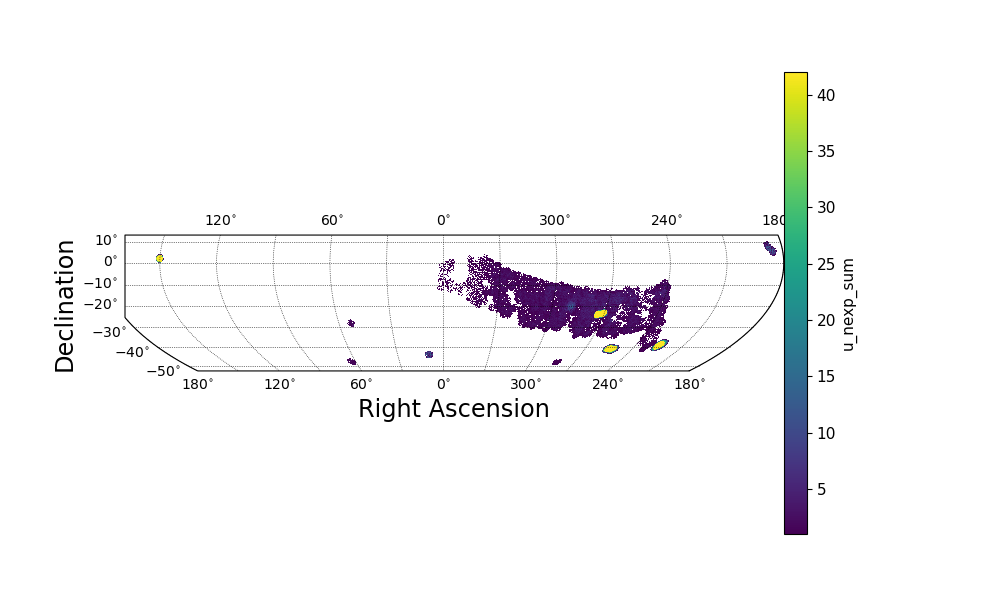
\includegraphics[width=\linewidth]{figures/expected_coadd_u_nexp_skyproj.png}
    \caption{$u$}
\end{subfigure}
\hfill
\begin{subfigure}{0.48\textwidth}
    \centering
    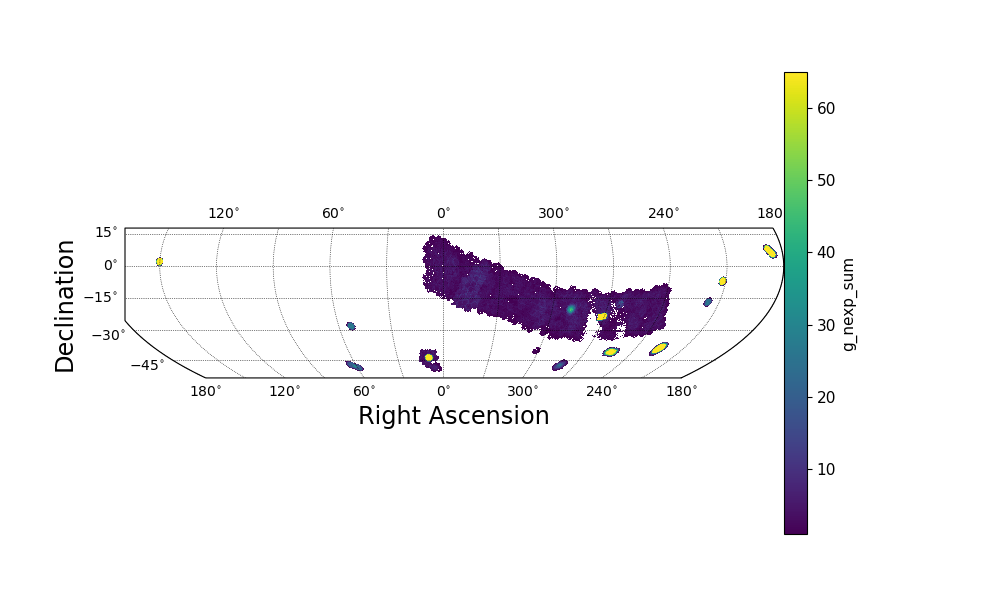
\includegraphics[width=\linewidth]{figures/expected_coadd_g_nexp_skyproj.png}
    \caption{$g$}
\end{subfigure}

\vspace{0.4cm}

% Row 2
\begin{subfigure}{0.48\textwidth}
    \centering
    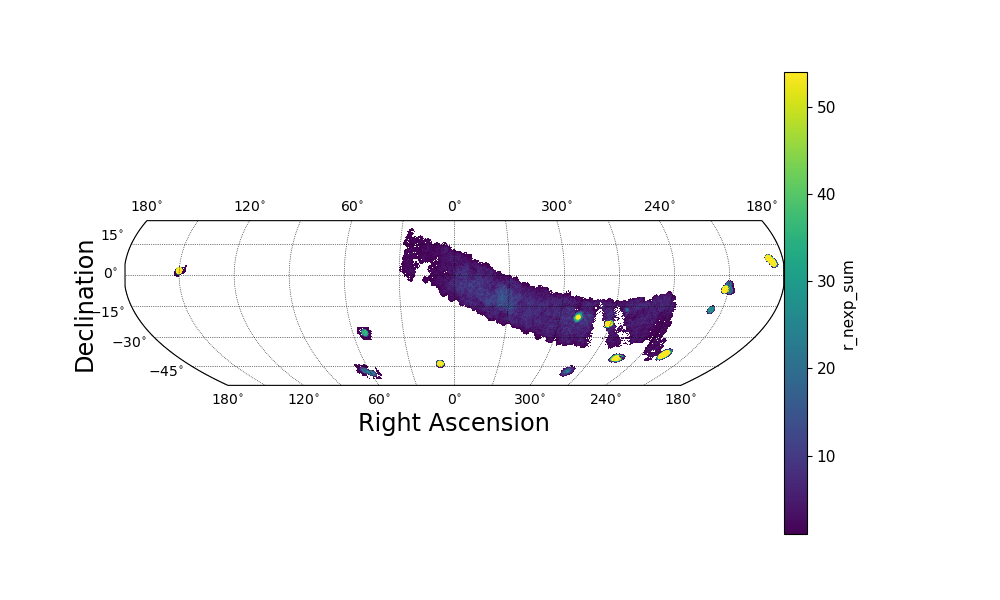
\includegraphics[width=\linewidth]{figures/expected_coadd_r_nexp_skyproj.png}
    \caption{$r$}
\end{subfigure}
\hfill
\begin{subfigure}{0.48\textwidth}
    \centering
    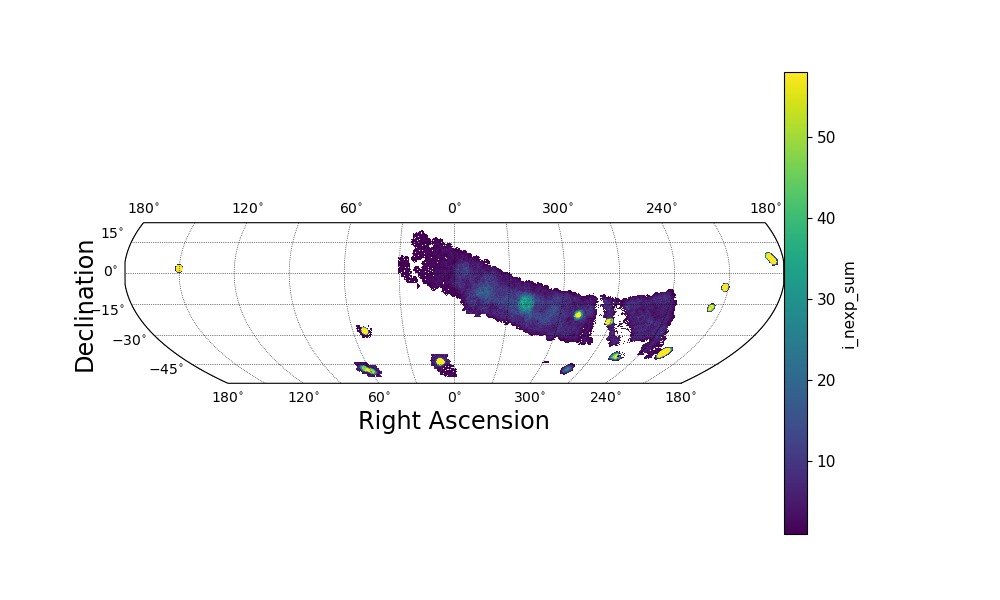
\includegraphics[width=\linewidth]{figures/expected_coadd_i_nexp_skyproj.png}
    \caption{$i$}
\end{subfigure}

\vspace{0.4cm}

% Row 3
\begin{subfigure}{0.48\textwidth}
    \centering
    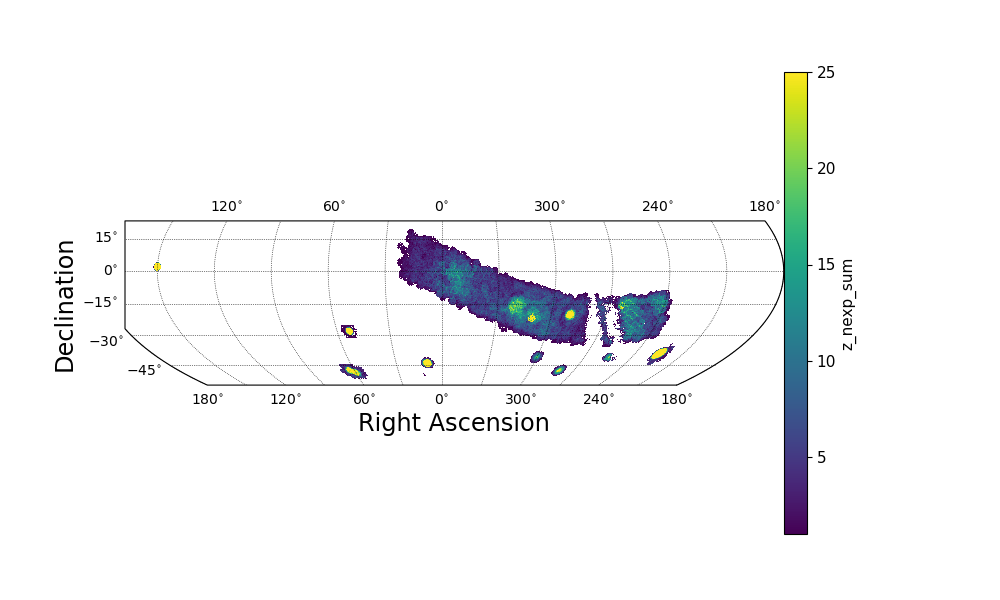
\includegraphics[width=\linewidth]{figures/expected_coadd_z_nexp_skyproj.png}
    \caption{$z$}
\end{subfigure}
\hfill
\begin{subfigure}{0.48\textwidth}
    \centering
    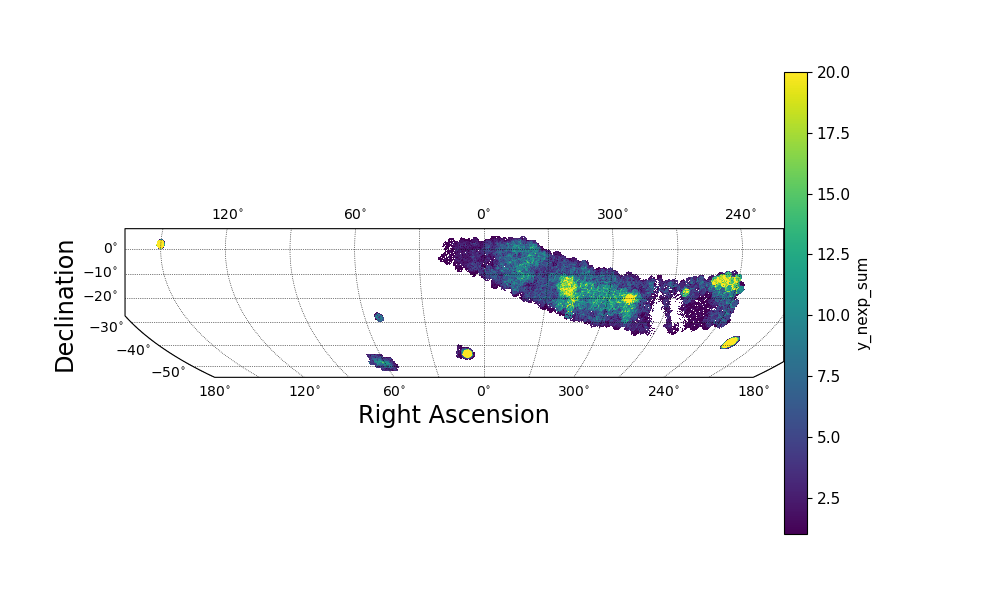
\includegraphics[width=\linewidth]{figures/expected_coadd_y_nexp_skyproj.png}
    \caption{$y$}
\end{subfigure}

\caption{PRELIMINARY EXPECTED DP2 number of input visits to coaddition in each LSST band (ugrizy) based on the QuickLook measurements in ConsDB.
Use table \ref{tab:coadd-visits-by-band-updated} to determine the number of
 visits contributing to deep drilling fields and field surveys taken during First Look.}
\label{fig:dp2_coadd_depth}
\end{figure*}
